\documentclass{article}
\usepackage{a4wide}
\usepackage[utf8]{inputenc}
\usepackage[T1]{fontenc}
\usepackage[french]{babel}
\usepackage[babel=true]{csquotes} % guillemets français
\usepackage{graphicx}
\usepackage{xcolor}
\usepackage{hyperref}
\usepackage{wrapfig}
\hypersetup{colorlinks,linkcolor=,urlcolor=blue}

\usepackage{amsmath}
\usepackage{amssymb}

\title{\textbf {\color{red} {Rapport de Projet Licence 3 Informatique :\\Présentation de l'application RunTourist}}}
\author{ {\color{cyan} Xavier Lacoudray 36005157 \\ \color{cyan} Sautron Samuel 36000990}}
\date{\itshape Avril 2021}

\begin{document}
\maketitle
\begin{abstract}

La Réunion terre d’outre-mer située entre terre et mer, préparez-vous à un voyage!
\newline
Résident ou même Touriste la Réunion regorge de Lieu dont nous ignorons, mais grâce à notre application vous pourrez découvrir ou redécouvrir ces Lieux Emblématiques. 
\end{abstract}

\section{\textcolor{brown}{Introduction }}
\label{section:intro}
{\color{magenta}\em{Quel projet avons-nous choisi de réaliser ?}}
\newline
\color{blue}Pour notre projet, on a choisi de créer une application orientée pour les Touriste ou Résident de la Réunion qui veulent se renseigner sur les lieux de notre île.
\newline \\
{\em\color{magenta}Pourquoi ce Projet d'application?}
\newline
\color{blue} Au départ on a voulu s’orienter sur une application de randonnées, car n’ayant pas trouvé d'application ou de site regroupant toutes les Randonnées de l'île on avait cette idée, mais la mise en place de cette application nous semble trop compliqué pour nos débuts en Développement mobile du fait de la gestion de coordonnée et de l'utilisation de Google Maps pour se repérer sur la Carte. On a décidé de partir sur une application plus simple dans le procédé, mais qui se rapporte toujours à notre idée de faire découvrir ou redécouvrir la Réunion.
\newline \\
{\em\color{magenta}Quelle est le but de l'application?}
\newline
\color{blue} Le but de l’application est de pouvoir regarder les différents lieux par rapport aux cardinalités de l’île (Nord, Sud, Ouest et Est) si le lieu intéressé l’utilisateur, il peut la sauvegarder dans mes favoris afin de se retrouver plus facilement l’application est facile d’accès.
L’utilisateur peut aussi supprimer ces favoris et grâce à la base donnée avoir une persistance des données.
\newline\\
Nous allons vous montrez les différents visuels de notre application l’utilisation sur Android, puis une description du Code, on continuera avec celle d’iOS ainsi nous finirons avec notre ressenti et l’avenir de notre application.

{\color{brown}\section{Description générale de l'application}}
\label{section:description}

{\color{olive}\subsection{Mode Portrait}}
\begin{minipage}{0.5\textwidth}
\subsubsection{\color{purple}Page d'accueil}
Voici l'écran d'accueil il comporte 5 boutons :
\begin{itemize}
 \item Le bouton Lieux a visité qui va afficher une nouvelle page pour choisir les lieux en fonction de leur cardinalité.
\item Le bouton Lieux Favorites qui permettra de stock sur une base de donnée locale les lieux qui nous intéresse.
\item Le bouton Lieux Favoris en bas à gauche (un raccourci menant directement sur la page Lieux Favorites).
\item Le bouton Home en tout en bas au milieu (un raccourci pour revenir a l'accueil).
\item Le bouton Lieux a visité en bas à droite (un raccourci pour revenir sur la page Lieux a visités).
\newline On a en bas une surbrillance sur le bouton home en bas qui nous indique ou on se trouve.  
\end{itemize}
\end{minipage}
\hfill
\begin{minipage}{0.3\textwidth}
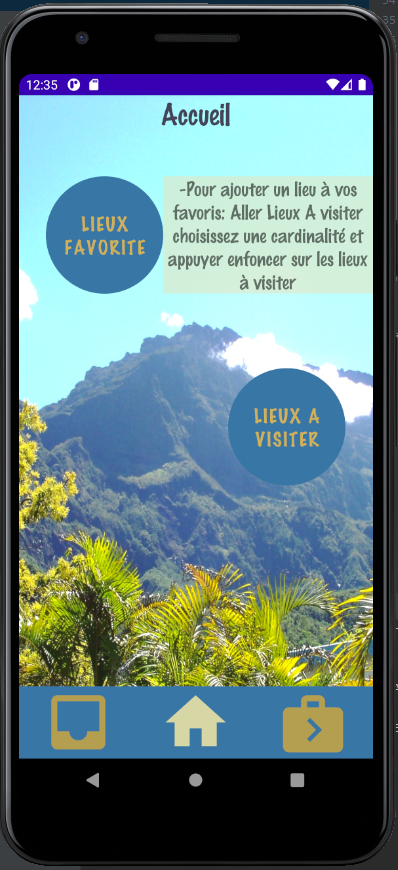
\includegraphics[width=\textwidth]{Acceuil}
\end{minipage}


\begin{minipage}{0.5\textwidth}
\subsubsection{\color{purple}Page lieux a visiter}
Voici l'écran des "Lieux à Visiter" il comporte 4 boutons :
\begin{itemize}
 \item Le bouton Nord qui ouvre une nouvelle page sur les lieux dans le nord de l'île.
 \item Le bouton Sud qui ouvre une nouvelle page sur les lieux dans le sud de l'île.
 \item Le bouton Ouest qui ouvre une nouvelle page sur les lieux dans l'ouest de l'île.
 \item Le bouton Est qui ouvre une nouvelle page sur les lieux dans l'est de l'île.
 \\ On a toujours une surbrillance sur le bouton en bas à droite nous indiquant qu'on est sur la page "Lieux À visiter"
\end{itemize}
\end{minipage}
\hfill
\begin{minipage}{0.3\textwidth}
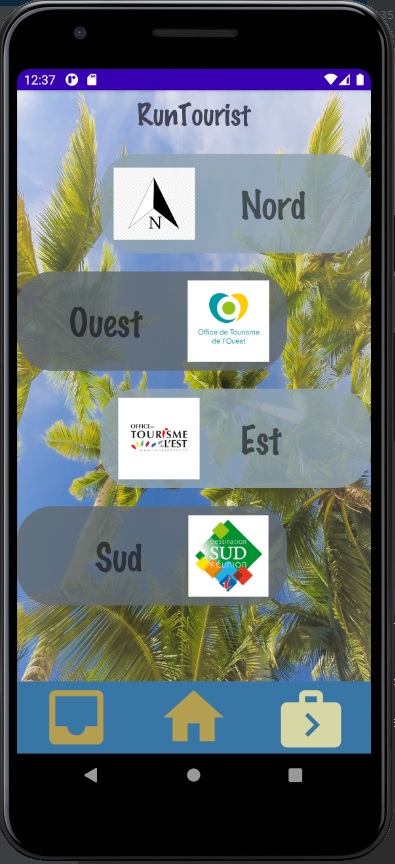
\includegraphics[width=\textwidth]{Lieux_a_visiter}
\end{minipage}

\subsubsection{\color{purple}Pages des cardinalités}
\begin{minipage}{0.23\textwidth}
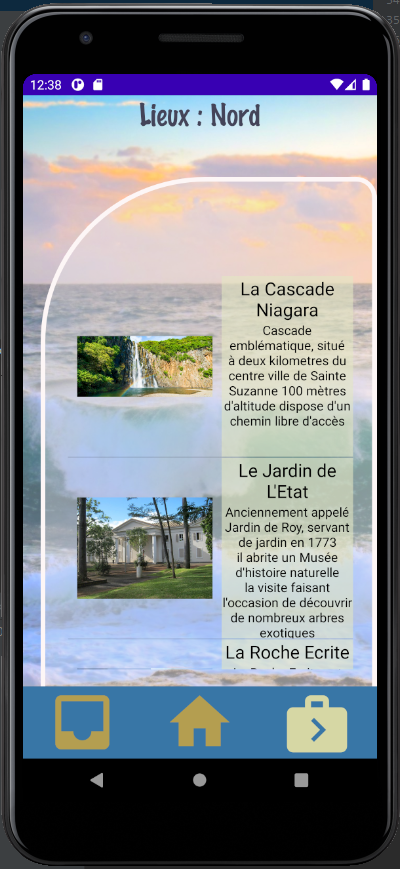
\includegraphics[width=\textwidth]{Lieux_nord}
\end{minipage}
\hfill
\begin{minipage}{0.23\textwidth}
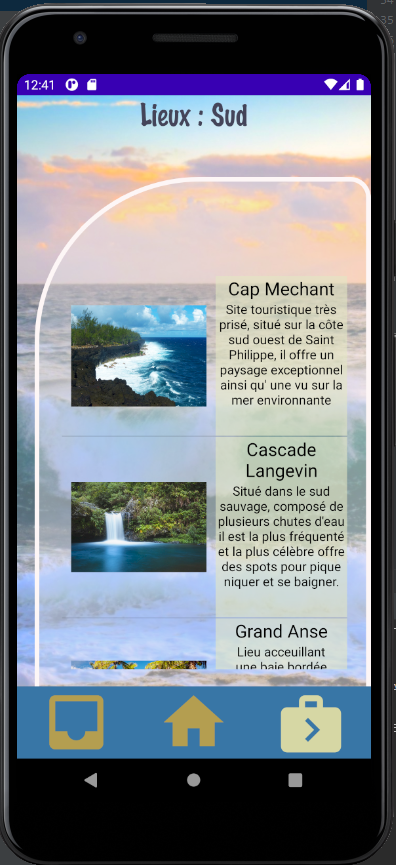
\includegraphics[width=\textwidth]{Lieux_sud}
\end{minipage}
\hfill
\begin{minipage}{0.23\textwidth}
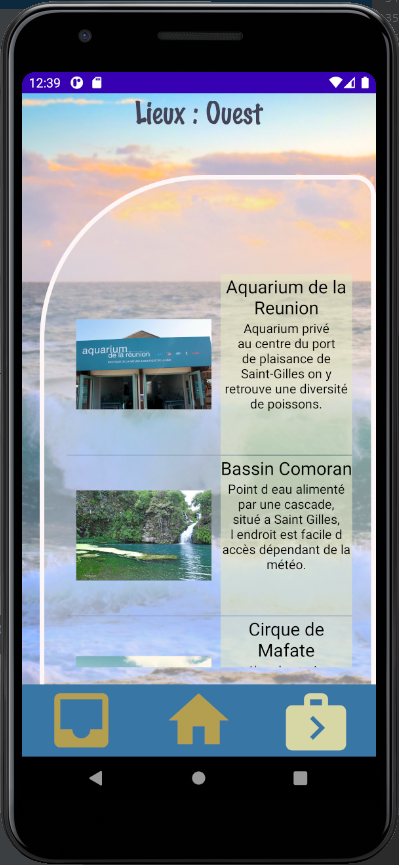
\includegraphics[width=\textwidth]{Lieux_ouest}
\end{minipage}
\hfill
\begin{minipage}{0.23\textwidth}
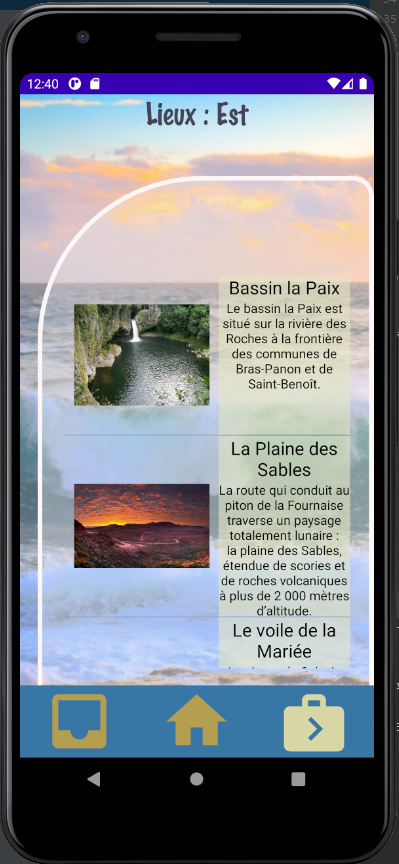
\includegraphics[width=\textwidth]{Lieux_est}
\end{minipage}
Nous avons ici les quatre cardinalités distinctes avec leur propre liste de lieux, ils ont cinq lieux au total. Pour sauvegarder un lieu intéressant il faut maintenir le clic sur la zone de la photo et du texte une réponse vous affichera qu'il à été bel et bien sauvegardé dans vos favoris.


\subsubsection{\color{purple}Page mes favoris}
\begin{minipage}{0.5\textwidth}
    
Nous avons maintenant 2 pages mes favoris l'un est vide pour l'instant et si on ajoute des lieux a sa base il deviendra comme la deuxième page une notification apparaîtra une fois qu'un lieu est enregistré. Il y a aussi 2 nouveaux boutons : \\

\begin{itemize}
    \item Le bouton "vider mes favoris" qui supprime touts les lieux enregistrer dans la base de données locale.
    \item Le bouton actionnable "supprimer" qui permet de supprimer un lieu de la base en maintenant le clic sur le lieu.
\end{itemize}
\end{minipage}
\hfill
\begin{minipage}{0.2\textwidth}
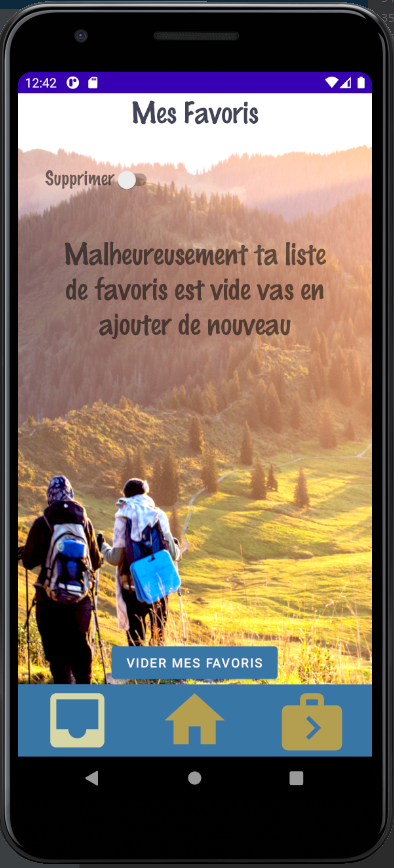
\includegraphics[width=\textwidth]{Mes_favoris_vide}

\end{minipage}
\hfill
\begin{minipage}{0.2\textwidth}
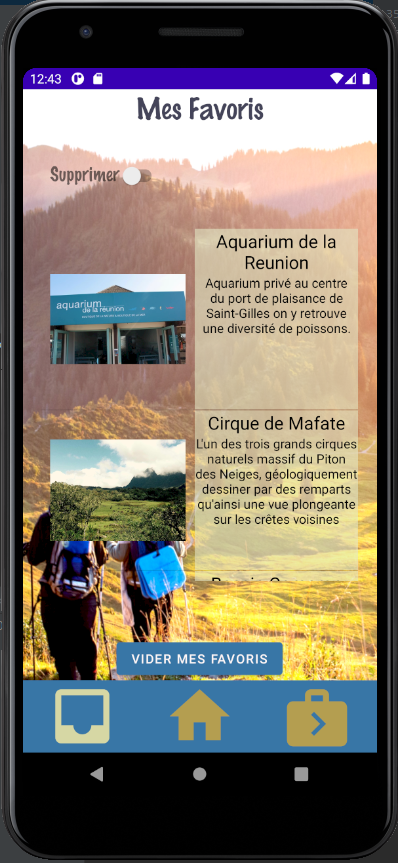
\includegraphics[width=\textwidth]{Mes_favoris}
\end{minipage}



{\color{olive}\subsection{ Mode Paysage}}
{\color{purple}\subsubsection{Page acceuil}}
\begin{minipage}{0.5\textwidth}
 Comparé a son mode normale, il n'y a vraiment pas de changement les boutons ont dus être réadapté en circonstance. 
\end{minipage}
\hfill
\begin{minipage}{0.4\textwidth}
    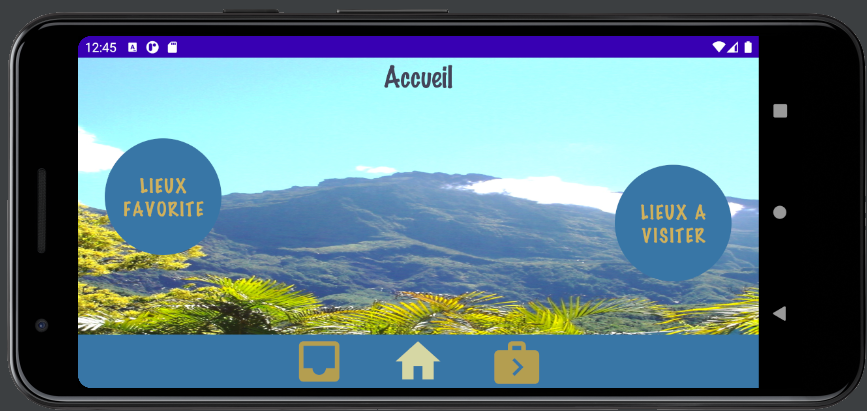
\includegraphics[width=\textwidth]{Acceuil_p}
    
\end{minipage}

{\color{purple}\subsubsection{Page lieux a visiter}}
\begin{minipage}{0.5\textwidth}
 Comparé a son mode normale, les boutons ont changé de place et sont devenues comme des colonnes. 
\end{minipage}
\hfill
\begin{minipage}{0.4\textwidth}
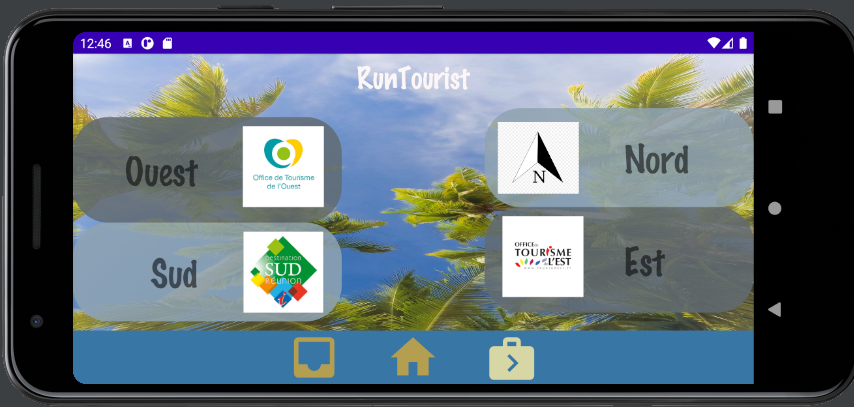
\includegraphics[width=\textwidth]{Lieux_a_visiter_p}
\end{minipage}
    
{\color{purple}\subsubsection{Pages des cardinalités}}
\begin{minipage}{0.45\textwidth}
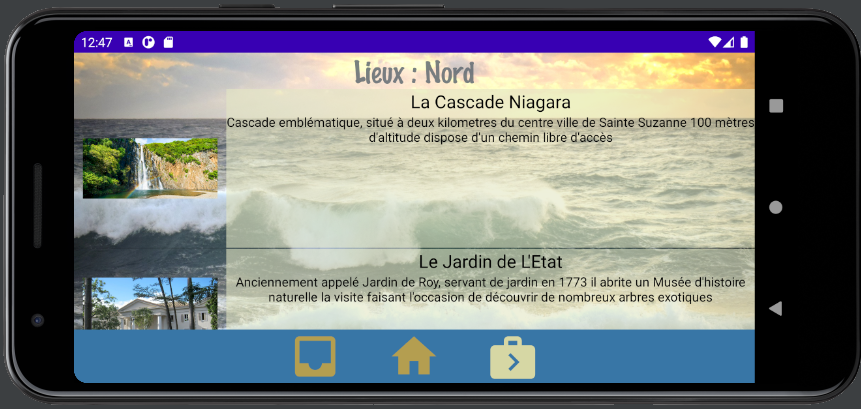
\includegraphics[width=\textwidth]{Lieux_nord_p}
\end{minipage}
\hfill
\begin{minipage}{0.45\textwidth}
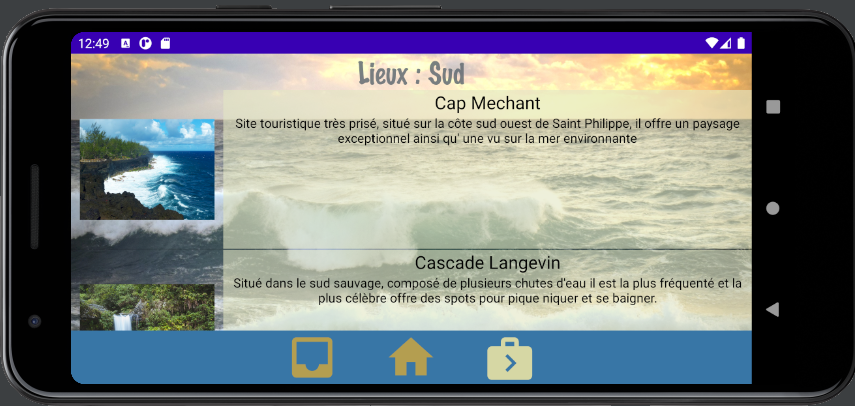
\includegraphics[width=\textwidth]{Lieux_sud_p}
\end{minipage}

\begin{minipage}{0.45\textwidth}
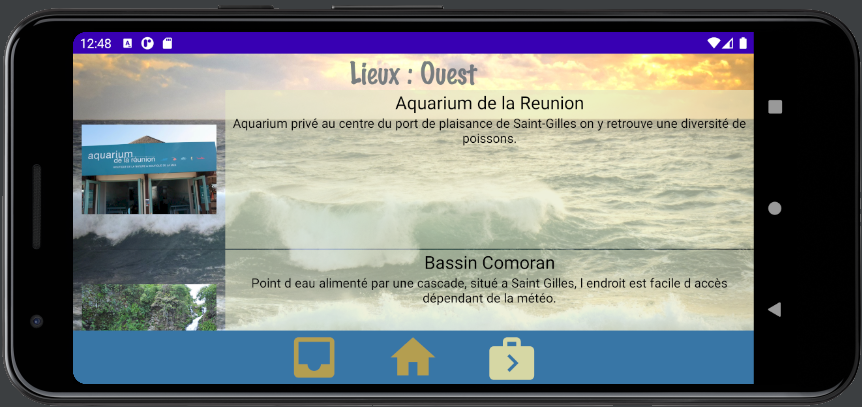
\includegraphics[width=\textwidth]{Lieux_ouest_p}
\end{minipage}
\hfill
\begin{minipage}{0.45\textwidth}
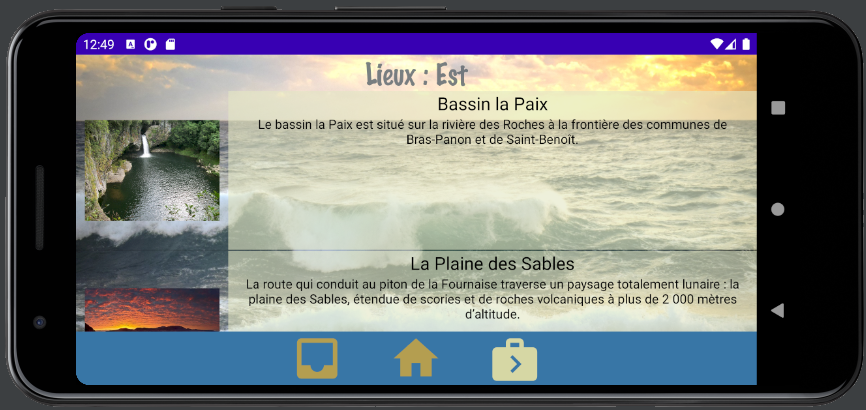
\includegraphics[width=\textwidth]{Lieux_est_p}
\end{minipage}
\\
On peut apercevoir qu'ici, c'est devenu plus petit il y a une perte d'informations qu'on ne puisse pas voir, mais avec un scrollview on peut néanmoins accéder aux autre parti caché de l'écran comme son prédécesseur en mode normale. 

{\color{purple}\subsubsection{Page mes favoris}}
\begin{minipage}{0.45\textwidth}
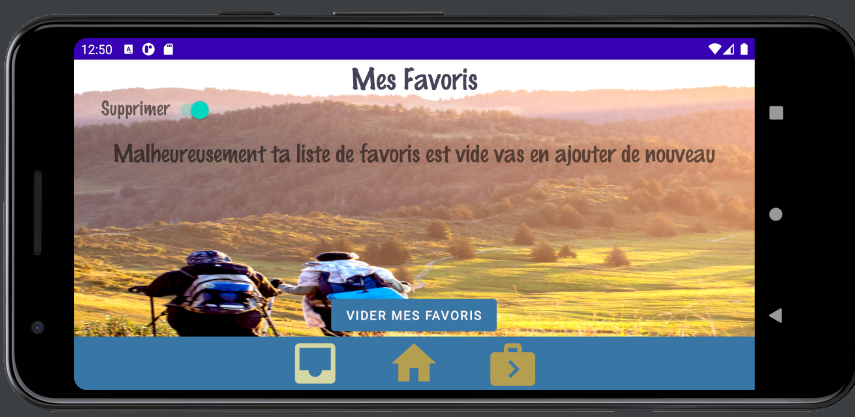
\includegraphics[width=\textwidth]{Mes_favoris_vide_p}
\end{minipage}
\hfill
\begin{minipage}{0.48\textwidth}
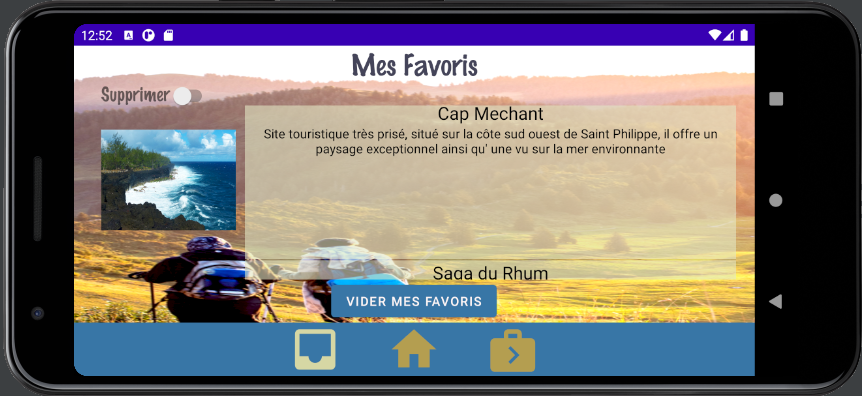
\includegraphics[width=\textwidth]{Mes_favoris_p}
\end{minipage}
Comme son prédécesseur, c'est la même chose sauf que peut juste voir l'affichage d'un seul lieu favori toujours accessible avec un scrollview le reste des lieux enregistrer. 

{\color{brown}\section{Code}}
\label{section:code}
{\color{olive}\subsection{MainActivity}}
\begin{minipage}{0.5\textwidth}
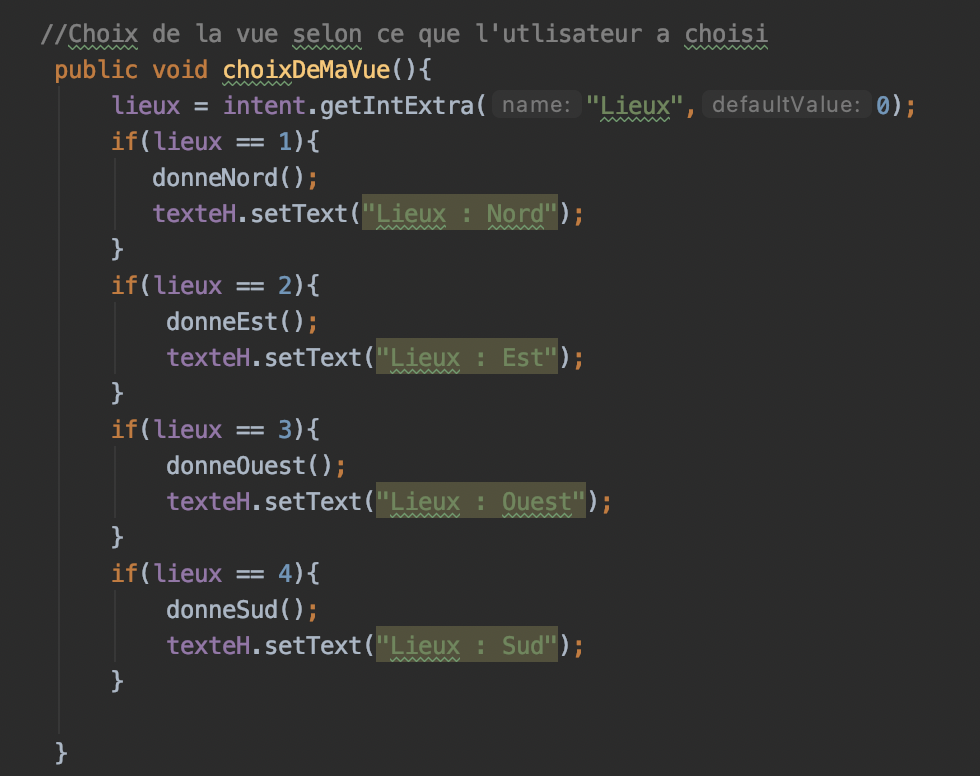
\includegraphics[width=\textwidth]{code1.png}
\end{minipage}
\hfill
\begin{minipage}{0.45\textwidth}
L’utilisateur commence tout d’abord sur une page d’accueil si ce lui vas dans les lieux a visité et arrive au 4 points cardinaux.
Il doit choisir une cardinalité qui sera interprété par la fonction choixDeMaVue dans le MainActivity2, on utilise ici un entier «lieu» selon ce que l’utilisateur décide de choisir il enverra un entier qui transféra les données a affiché dans la ListView.
\end{minipage}
{\color{olive}\subsection{AffCell}}
\begin{minipage}{0.9\textwidth}
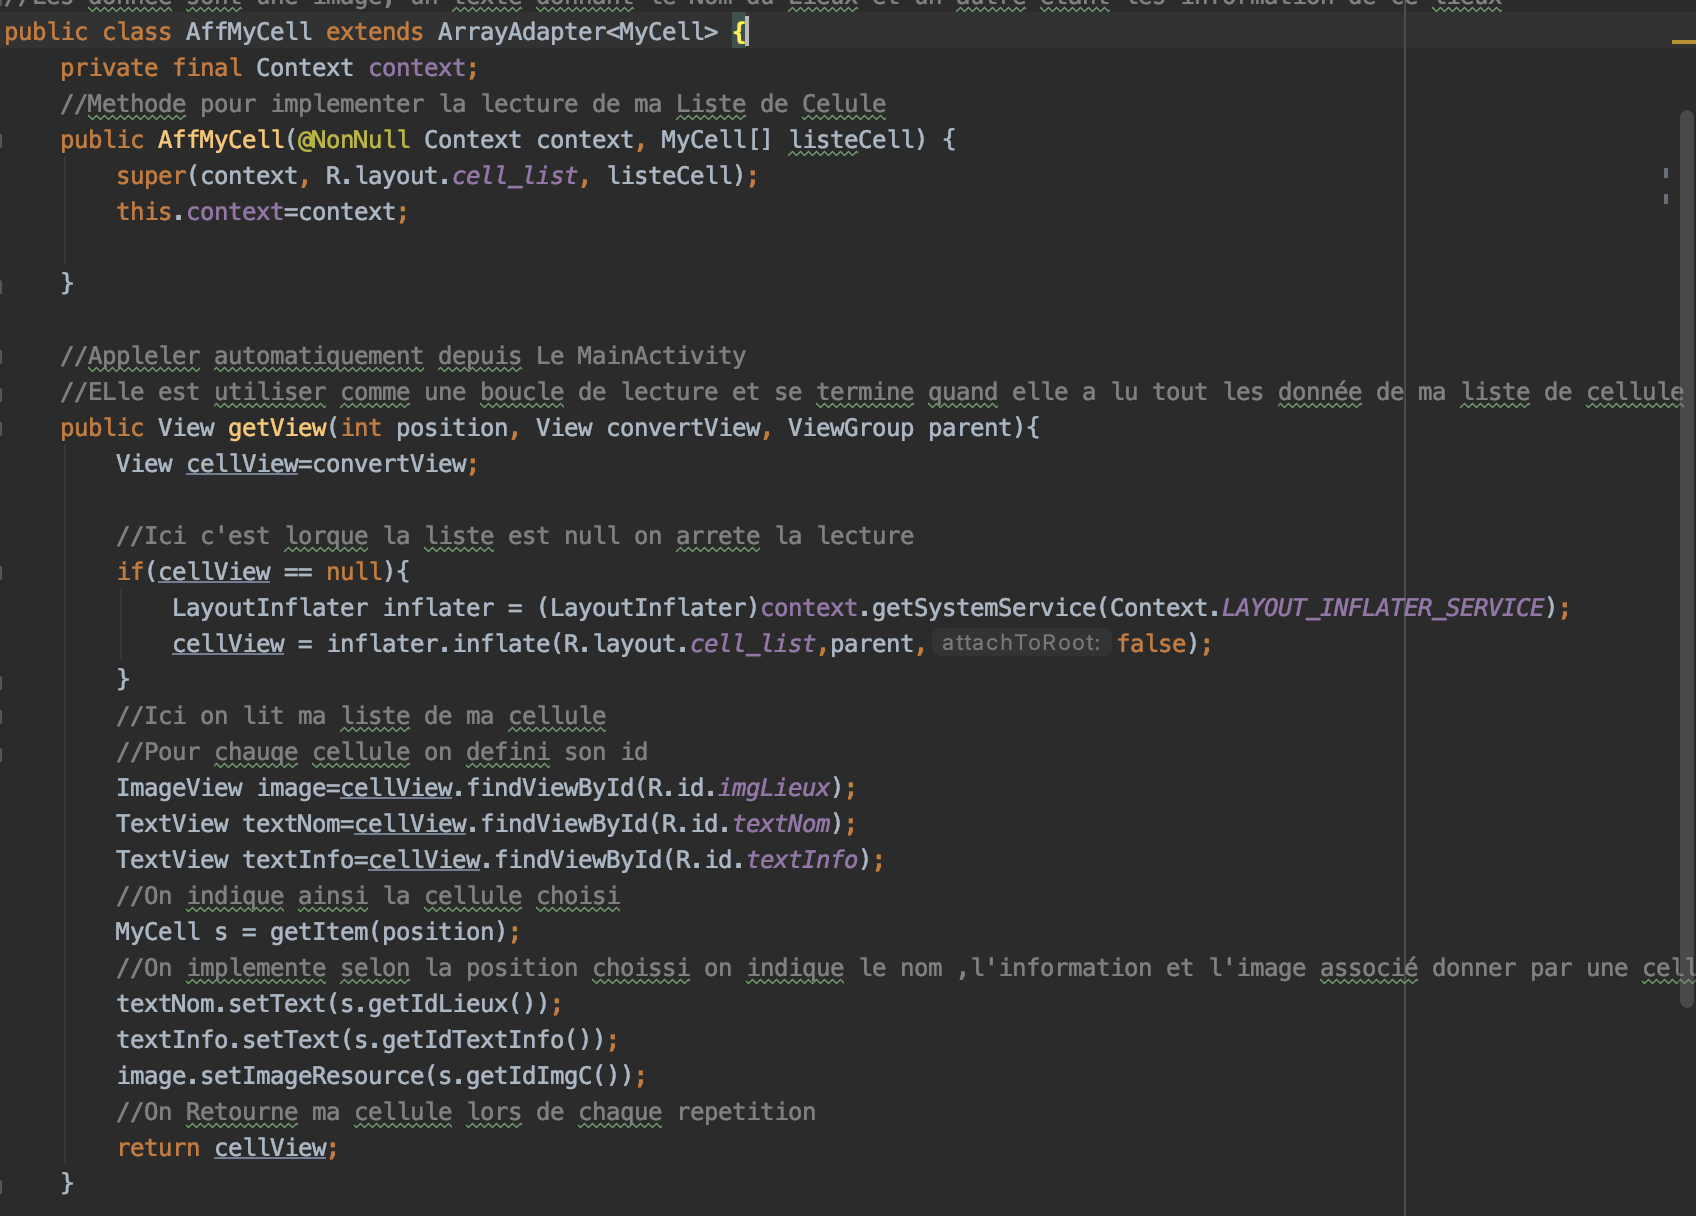
\includegraphics[width=\textwidth]{code2.png}
\end{minipage}
\\
Pour afficher correctement la listeraient d’envoyer les données choisies plus haut est affiché dans cette ListView, on a la fonction getView qui se démarre automatiquement pour lire la liste de nos lieus, celle-ci fonctionne comme une boucle et fini quand la liste sera vide ainsi a chaque passage on donne l’image, nom du lieu et les informations complémentaire à afficher dans la cellule.
{\color{olive}\subsection{MainActivity2}}
\begin{minipage}{0.9\textwidth}
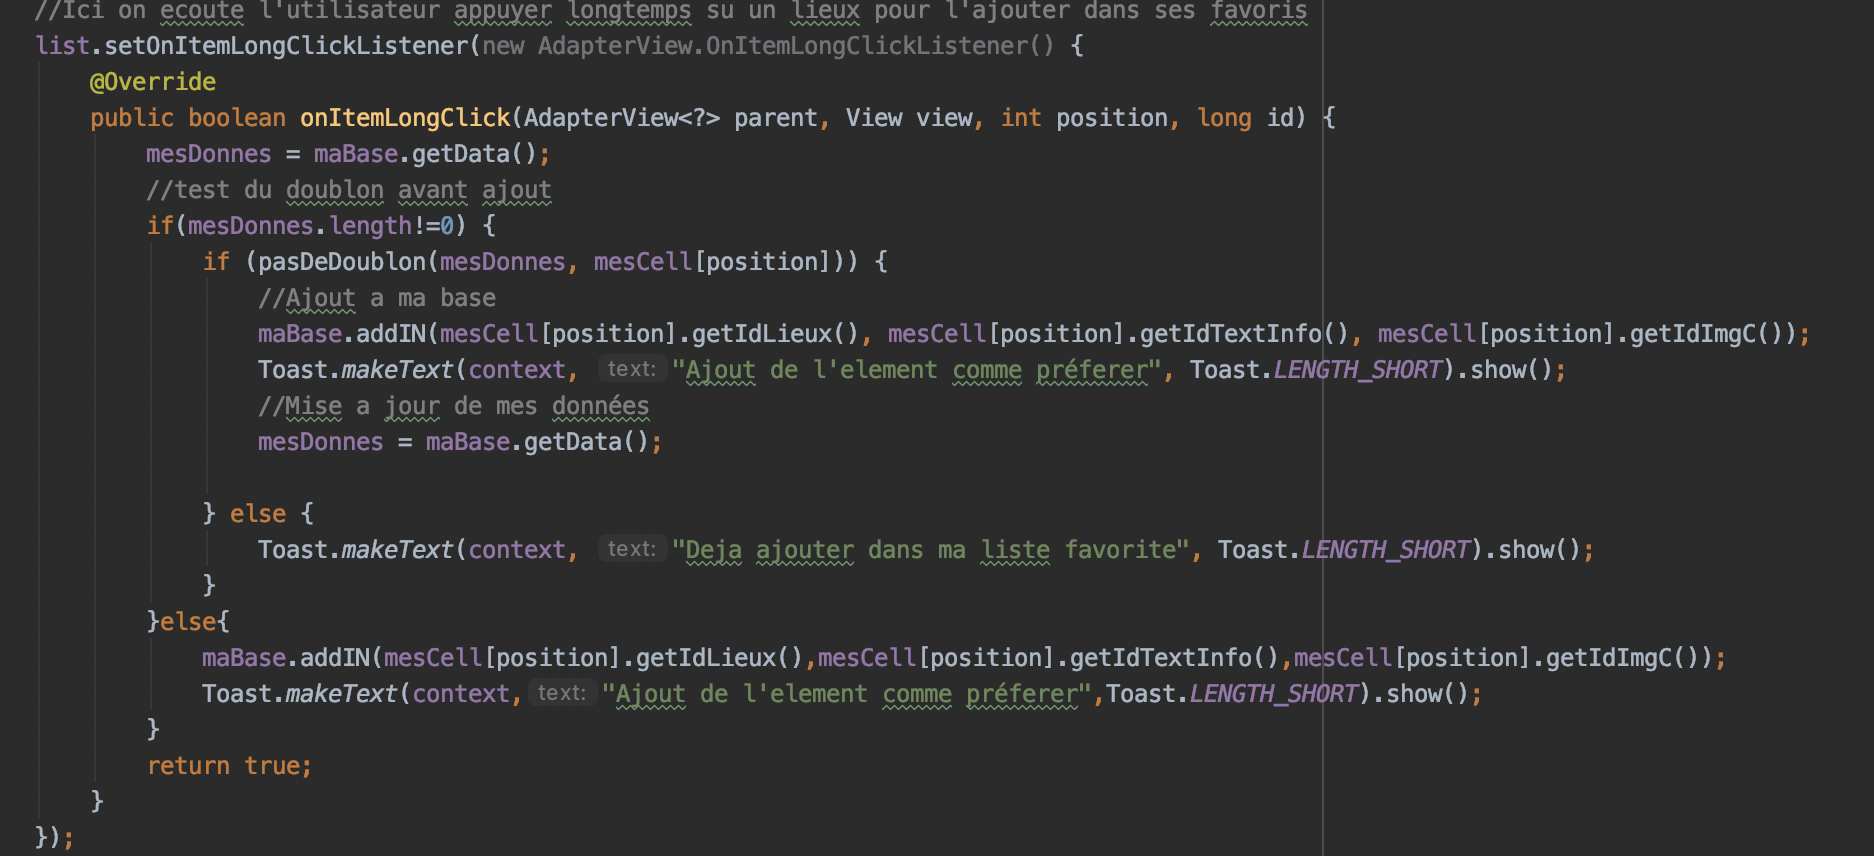
\includegraphics[width=\textwidth]{code3.png}
\end{minipage}
\\
Lorsque l’utilisateur appuie enfoncé sur un lieu celle-ci envoye un message et Ajoute à la base de donnée notre élément choisi. On envoye dans la base donnée la position «servant à supprimer», et les données propres aux lieux Image, Nom et Info.
On remarque aussi la Fonction pas de doublon pour éviter les doublons dans ma liste Favorite.
\subsection{ \color{olive} Base de Donnée}
\begin{minipage}{0.7\textwidth}
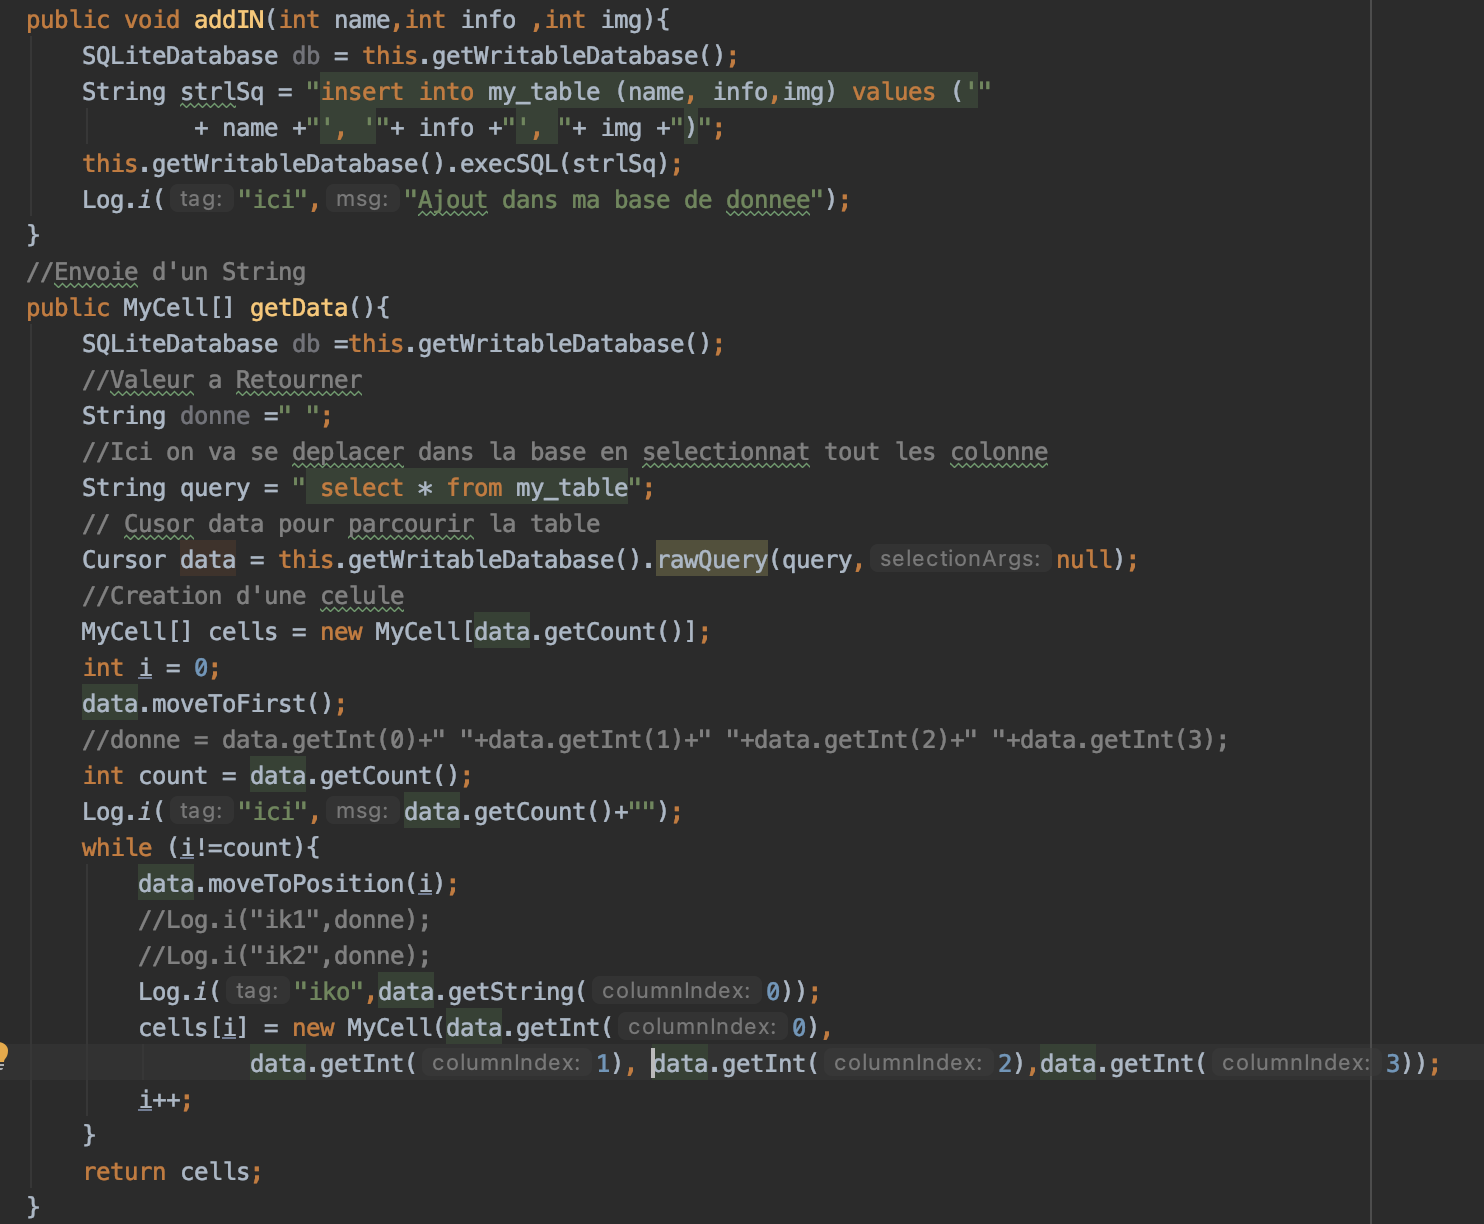
\includegraphics[width=\textwidth]{code4.png}
\end{minipage}
\\
\\
Ici ce sont les fonctions servant à ajouter les informations d’un lieu choisi par l’utilisateur dans une base donnée est ainsi de la sauvegarder.
La fonction addIN ajoute un lieu et pour afficher les lieux on a getData.
La Fonction getData renvoie un une liste de MyCell contenant tous les Lieus choisis par l’utilisateur.
Pour parcourir la Table on écrit en SQL "select * from my table"
que je vais directement transfère chaque information qui sont classés par colonne dans ma cells selon l’indice qui est incrémenté au fur et a mesure par «i».
À la fin on retournera cells comportant les lieus choisis par l’utilisateur.

{\color{brown}\section{Parti iOS}}
\begin{minipage}{0.4\textwidth}
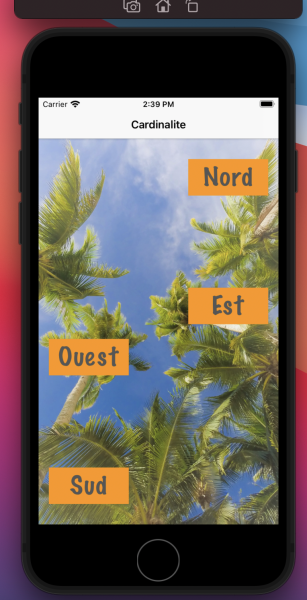
\includegraphics[width=\textwidth]{ios1.png}
\end{minipage}
\begin{minipage}{0.25\textwidth}
Ici si on appuie sur Nord
\end{minipage}
\begin{minipage}{0.4\textwidth}
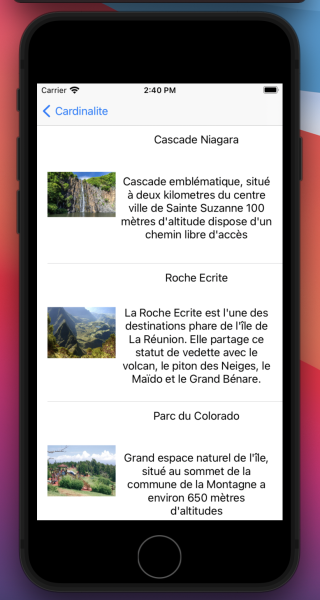
\includegraphics[width=\textwidth]{ios2.png}
\end{minipage}
On a donc la même fonctionnalité que la version Android selon la cardinalité choisie on a accès a la liste des différents lieux.
On a rencontré des problèmes avec la version iOS dû au fait de l'affichage soit celle de régler les contraintes pour avoir le même affichage que celui d'Android.
On a aussi eu du mal avec iOS ne pas tout coder simplement comme sur Android studio et n’ayant pas le même type de langage nous a posé problème.
\newline
Certes malgré les problèmes on a réussi avoir une application basique  sans les fonctionnalités favoris.

 



{\color{brown}\section{Conclusion}}
\label{section:conclusion}
Notre Application est donc fonctionnelle que ce soit sur Android ou sur iOS, on est fiers de vous la présenter. On a appris vis-à-vis de ce projet que créer une application n'est pas simple et demande beaucoup de rigueur en termes de travail et aussi en termes de travail personnel. On a su malgré tout structurer notre projet.
Seulement on n’a pas pu passer assez de temps sur la partit iOS ou on voulait avoir les mêmes fonctionnalités comme "mes favoris" ou "la persistance de donnée".
Le Monde peut donc découvrir les lieux a visité à la Réunion grâce à notre application et c'est ça qui nous satisfait le fais d'être allé au bout de ce projet.
\\
Nos idées dans le futur ? 
Continuer l'application la rendre responsive et compatible a tout les téléphone. Mettre l'application iOS au même niveau que l'application Android. Pouvoir aussi utiliser Google Maps et la géolocalisation de son téléphone pour rechercher directement sur la Carte les Lieux.
Ajout aussi de Compte permettant à chaque Utilisateur de se connecter et avoir sa propre base sauvegarder en Ligne.




{\color{brown}\section{References}}
\label{section:references}
{\color{violet}\itshape Photos prises sur ces sites : }
\begin{itemize}
    \item \url{https://www.cartedelareunion.fr/listings/roche-ecrite}
    \item \url{https://www.zotcar.com/blog/cascade-la-reunion/}
\item \url{https://www.istockphoto.com/fr/search/2/image?phrase=cascade+niagara+\%C3\%AEle+de+la+r\%C3\%A9union}
\item \url{https://laterreestunjardin.com/jardin-etat-reunion/}
\item \url{https://www.cartedelareunion.fr/listings/parc-du-colorado}
\item \url{https://randopitons.re/tourisme/364-parc-loisirs-colorado}
\item \url{https://blog.tropicalhome.fr/vanilleraie-a-la-reunion/}
\item \url{https://www.cartedelareunion.fr/listings/piton-des-neiges}
\item \url{https://www.lechotouristique.com/article/crise-a-la-reunion-les-recommandations-du-seto/ile-de-la-reunion-cascade-langevin-2}
\item \url{http://espirituaventura.canalblog.com/archives/2012/10/30/25461287.html}
\item \url{https://www.lrphotographies.com/media/6295da75-6710-498d-a0db-effdc94fc776-explosion-de-vague-au-cap-mechant-saint-philippe}
\item \url{https://www.cartedelareunion.fr/listings/cap-mechant}
\item \url{https://orkymel.fr/petite-ile/la-plage-a-voir-a-la-reunion/}
\item \url{https://www.cartedelareunion.fr/listings/plage-de-grande-anse}
\item \url{https://www.cartedelareunion.fr/listings/saga-du-rhum}
\item \url{https://www.cartedelareunion.fr/listings/cirque-de-mafate}
\item \url{https://www.airfrance.fr/FR/fr/common/travel-guide/le-fantastique-piton-maido.htm}
\item \url{https://www.cartedelareunion.fr/listings/le-maido}
\item \url{https://blog.tropicalhome.fr/kelonia/}
\item \url{https://www.cartedelareunion.fr/listings/kelonia}
\item \url{http://gorgebleue.canalblog.com/albums/a1___la_reunion___paysages/photos/60011707-bassin_cormoran_tres_joli.html}
\item \url{https://blog.tropicalhome.fr/les-bassins-de-saint-gilles/}
\item \url{https://www.tripadvisor.fr/LocationPhotoDirectLink-g298470-d3349640-i77462278-Aquarium_de_la_Reunion-Saint_Gilles_Les_Bains_Arrondissement_of_Saint_Pau.html}
\item \url{https://www.cartedelareunion.fr/listings/piton-de-la-fournaise}
\item \url{https://dailygeekshow.com/cascade-legende-reunion/}
\item \url{https://www.rentiles.fr/blog-voyage/decouvrez-le-voile-de-la-mariee-a-la-reunion.html}
\item \url{https://www.cartedelareunion.fr/listings/voile-de-la-mariee}
\item \url{https://www.geocaching.com/geocache/GC7XX0Z_ec-la-plaine-des-sables?guid=3b9bc1e0-9e42-437f-bb95-ab7ab23764de}
\item \url{https://www.cartedelareunion.fr/listings/plaine-des-sables}
\item \url{http://www.lareunionparadis.com/les-10-choses-a-faire-absolument-dans-l-est-a-la-reunion/}
\item \url{https://www.cartedelareunion.fr/listings/le-bassin-la-paix-et-bassin-la-mer-depuis-abondance}
\item \url{https://www.cartedelareunion.fr/listings/eglise-notre-dame-des-laves}
\item \url{https://www.wlaps.com/notre-dame-des-laves-la-reunion/}

\end{itemize}




\end{document}
